\documentclass{article}

% Packages
\usepackage{amsmath}    % For math environments
\usepackage{graphicx}   % For including graphics
\usepackage{caption}
\usepackage{hyperref}   % For hyperlinks
\usepackage{listings}   % For code listings
\usepackage{geometry}   % To set page dimensions
\usepackage{wrapfig}

\usepackage{fancyhdr}   % For custom headers/footers
\usepackage{parskip}    % For paragraph spacing
\usepackage{enumitem}   % For better itemize/enumerate spacing
\usepackage{hyperref}   % For Hyper links
\usepackage{gensymb}    % symbols
\usepackage{siunitx}    % SI units
\usepackage{physics}    % For matrices and physics notation
\usepackage{cancel}     % add a diagonal mark to cross out an equation
\usepackage{biblatex}

\addbibresource{MyLibrary.bib}
\geometry{a4paper, margin=2.5cm}

\renewcommand{\topfraction}{.8} %how big can a float be at the top as a fraction of total page height
\renewcommand{\floatpagefraction}{.8}%how big can a float be as a fraction of total page height. Need to set both to allow large figures.

\begin{document}


% To do: A bit about Operators (functions) versus panels (UI elements)
% add more prose about number formatting
% Write section about scaling

% Moment arm computation validation figure
% body segment property validation figure



% Figures to add:
% Maybe intro overview figure?
% MuSkeMo Blender panels
% Collections in the outliner
% Custom properties screenshot
% Screenshot of each panel?

% Modifier panel User inputs

% User settings of the muscle viewer node
% Presets in the expansions panels
% User modifiable inputs in the muscle visualization nodes.
% Examples of volumetric muscle visualizations



% Before / after picture of recommended render settings
% Before / after with black falloff
% Comparison picture evee cycles

% OpenSim converter Script screenshot
% Line of action Fitter screenshot

% Wrapping figures.

% Manually creating the title page
\begin{center}
    {\huge \textbf{MuSkeMo Manual}}\\[20pt]  % Title
    \vspace{10pt}  % Space between title and image

    \begin{figure}[h]
        \centering
        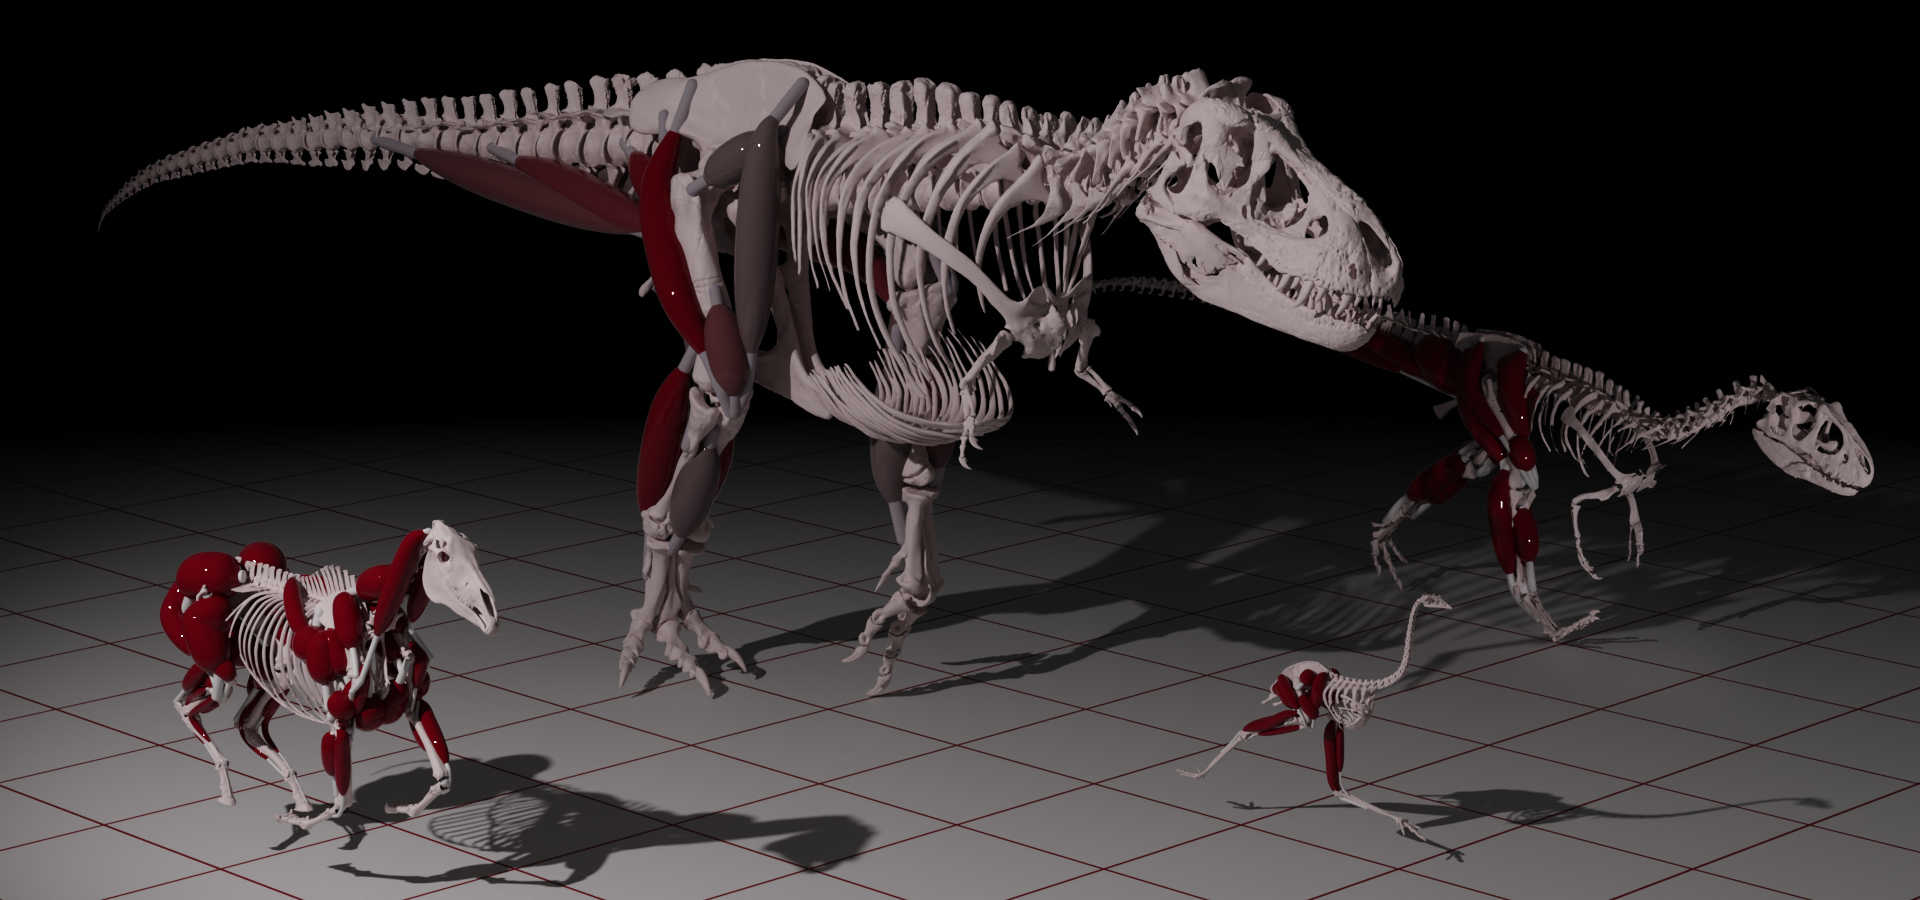
\includegraphics[width=\textwidth]{figures/cover_pic.png} % Add image
    \end{figure}
    \setcounter{figure}{0}
    \vspace{20pt} % Add vertical space between image and author section
    
    {\Large \textbf{Pasha van Bijlert}}\\
    \vspace{10pt}
    \textbf{pashavanbijlert@gmail.com}\\
    \textbf{Github Repository:} \href{https://github.com/PashavanBijlert/MuSkeMo}{Github} \\
    \textbf{Bug Reports and Feature Requests:} \href{https://github.com/PashavanBijlert/MuSkeMo/issues}{Submit an issue on Github} \\
    \vspace{20pt}
    {\large Version 0.9.1} \\
    {\large \today}
\end{center}

\vfill  % This pushes the content to the bottom of the page

\newpage  % Page break to separate the title page from the rest of the document


\tableofcontents

\newpage
\section{Introduction}

MuSkeMo is a tool for musculoskeletal modeling in \href{https://www.blender.org}{Blender}. MuSkeMo allows you to translate biological 3D scans to useful biomechanical information, in the form of full models or model components. These can then be used for further analysis within Blender, or exported for simulations in other biomechanical software. Simulation trajectories can be imported back into MuSkeMo to make publication-ready stills and videos, using Blender’s built-in raytracing rendering. MuSkeMo can also be used for 3D landmarking and for simply calculating inertia tensors from 3D scans.

This MuSkeMo documentation file is meant to complement the \href{https://www.youtube.com/watch?v=9eMm9YalXtg&list=PLfgxaucAWlEp5-cavvXmdrTIWYT_tgZYK&pp=gAQBiAQB}{video tutorial series on YouTube}.
This documentation is focused on features specific to MuSkeMo, and where necessary provides suggestions regarding Blender settings and features. Because Blender can be overwhelming at first, new users are recommended to follow the "Donut tutorial" series by BlenderGuru on Youtube. For Blender-specific questions, the reader is referred to the extensive \href{https://docs.blender.org/}{Blender documentation}. MuSkeMo currently officially supports Blender versions 3.0-4.1, but will offer 4.2+ support in the future. 

\section{Installation instructions}

To download: Go to the \href{https://github.com/PashavanBijlert/MuSkeMo/releases}{releases page} on the Github repository, and download the most recent version of "MuSkeMo.zip". The .zip file is used to install the plugin, but also contains a folder with utility functions (e.g., for OpenSim conversion).

To install (Fig. \ref{fig:installation}): In Blender v3-v4.1, go to Edit → preferences → Add-ons and then click "Install...", and then select your downloaded zip file. Then type in "MuSkeMo" in the search bar of the addon window, and enable the plugin by pressing the check mark. If using Blender 4.2+, you may need to use the legacy installer, but MuSkeMo has currently not been tested above v4.1.

\begin{figure}[h]
    \centering
    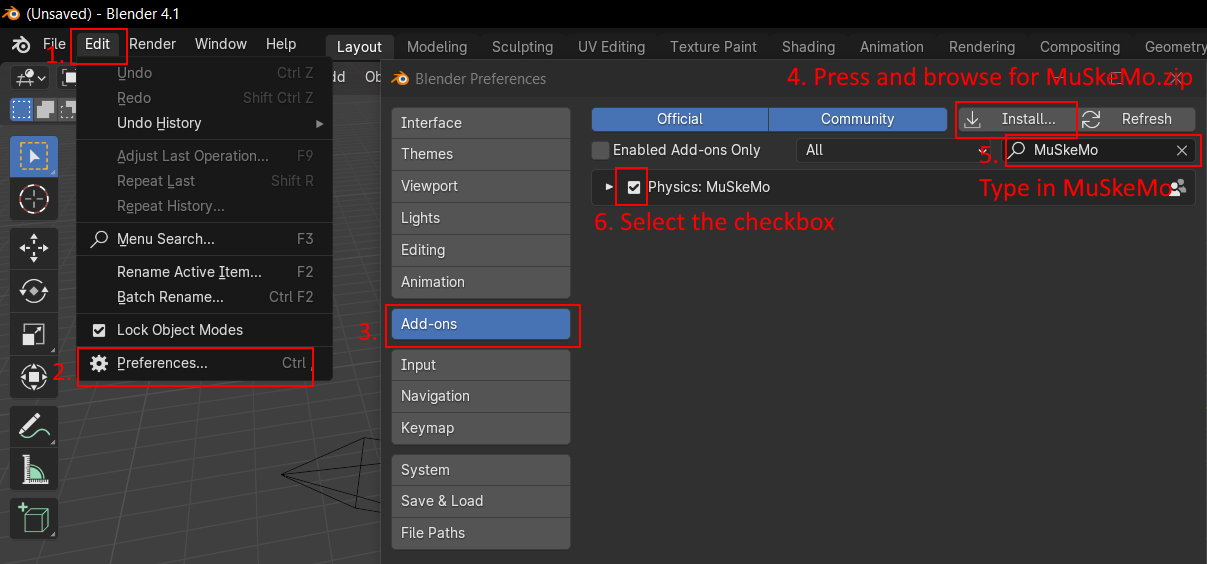
\includegraphics[width=\textwidth]{figures/install_instructions.png} % Add image
    \caption{Installing MuSkeMo in Blender versions 3.0-4.1}
    \label{fig:installation}
\end{figure}

\section{Units}

MuSkeMo uses the following units:

\begin{itemize}
    \item \textbf{Spatial distance/position:} metres (\si{\metre})
    \item \textbf{Mass:} kilogram (\si{\kilogram})
    \item \textbf{Moment of inertia:} kilogram metre squared (\si{kg\,m^2})
    \item \textbf{Force:} Newton (\si{N})
    \item \textbf{Angle:} Degrees (\si{\degree}, only for pennation angle). Internally MuSkeMo uses radians during computations.
\end{itemize}

\textbf{WARNING:} Blender's default units are in metres. Many of the calculations in MuSkeMo are derived from the spatial position of individual points (vertices) of the 3D meshes. If you change the base units of Blender, these calculations are also implicitly scaled, and the units will no longer be correct (e.g., if you change Blender’s base units to centimetres, linear dimensions will be off by a factor of 100, but volumetrics and inertial properties will be off by a factor of 100\(^3\)). MuSkeMo currently only officially supports metres as the base unit, correct scaling of the outputs if using other units is up to the user.

\section{A Note on Precision}
\label{sec:precision}

MuSkeMo is built using the Blender Python API, which internally uses double precision numbers (64-bit floating point, \(\sim16\) significant digits). However, Blender itself stores numbers using single precision (32-bit floating point, \(\sim8\) significant digits), including all 3D point and mesh data. This means that precision beyond 8 significant digits cannot be expected when using MuSkeMo. Single precision floats nevertheless have a very large range of numbers that can be represented—the smallest number that can be accurately reported is in the order of \(1\times10^{-38}\), approximately 1 million times smaller than the mass of an electron in kilograms.

Because computing inertial properties from 3D vertex data involves successive multiplications of single precision numbers, mass and inertial properties have an expected accuracy of 5-6 digits (see \ref{sec:inpropvalidation}).

\section{Orientations}

Orientations are represented as XYZ body-fixed Euler angles (see Appendix \ref{sec:eulerangles}) and as unit quaternions (see Appendix \ref{sec:quaternions}). Internally, MuSkeMo avoids Euler angles where possible because they are prone to gimbal lock, but popular simulators often use Euler angles by default (e.g., OpenSim, SCONE).


\section{Using MuSkeMo}

MuSkeMo lives in \href{https://docs.blender.org/manual/en/latest/interface/window_system/tabs_panels.html}{Blender panels} (Fig. \ref{fig:MuSkeMoUI}A). Panels can be interactively resized and collapsed, which can be useful depending on your screen size. Although Blender does support using a trackpad, it is substantially more intuitive to navigate with a mouse, and a keyboard with a separate numberpad. There are also certain settings that make navigation easier (see Section \ref{sec:MSM_glob_settings}).


\textbf{WARNING:} Ensure that 3D meshes (visual geometry and tissue outlines) have all their transformations applied before you start constructing the model. To do this, select the object, press \texttt{Control + A}, and select “All transforms”. This accounts for the way that Blender stores local transformations. When you move, rotate, and/or scale 3D models in Blender, these transformations are initially stored only locally in the object’s data (an extra storage layer in Blender). This means that the object’s position has not changed in 3D space, you have defined an extra local transformation that can easily be undone. Some of the functions in MuSkeMo may behave unpredictably unless transformations have first been applied.



\begin{figure}[htbp]
    %\vspace{-155pt}
    \centering
    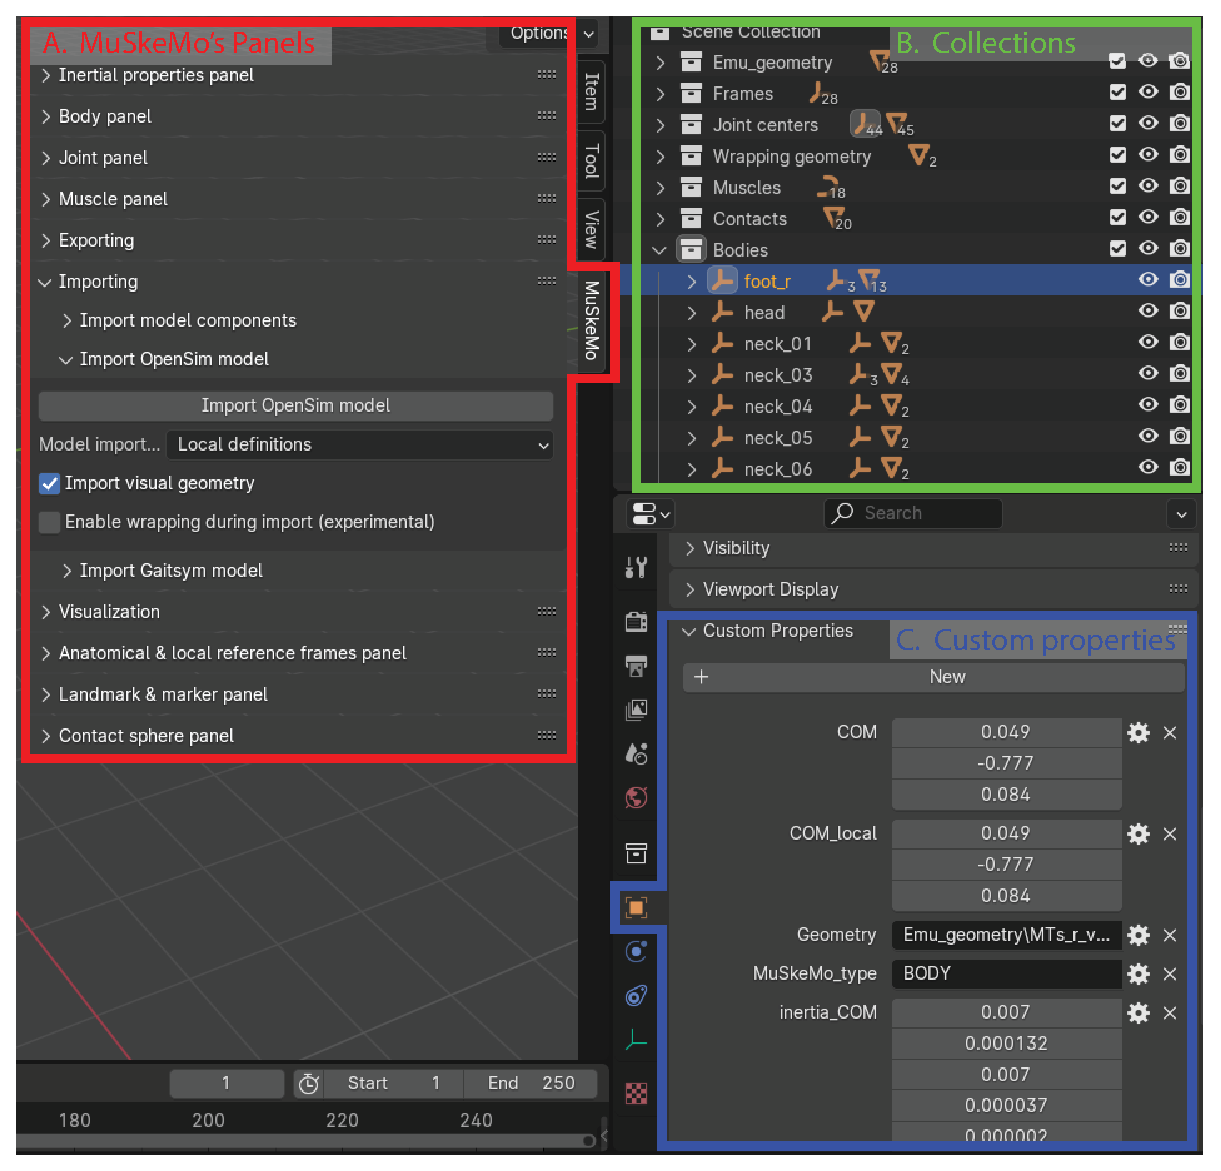
\includegraphics[width=0.99\textwidth]{figures/panels_coll_props.eps} % Add image
    \caption{A. All of MuskeMo's functionality can be accessed via these panels. The panels can be interactively resized and collapsed. B. After creating or importing model components, they are stored in Blender collections. If child objects are not visible, turn off object children in the outliner filter (see Section \ref{sec:MSM_glob_settings} C. A component's data are stored as custom properties. Press the yellow square, scroll all the way down, and open the Custom Properties dropdown}
    \label{fig:MuSkeMoUI}
\end{figure}

\subsection{Where MuSkeMo stores model data}
\label{sec:muskemodata}
All the model components and other user-created objects are stored in Blender \href{https://docs.blender.org/manual/en/latest/scene_layout/collections/collections.html}{Collections} (Fig. \ref{fig:MuSkeMoUI}B), which are essentially just folders. The collection names all have sensible defaults in MuSkeMo (e.g., "Bodies" for bodies), but can be changed if desired. The collection names are also used as the default filenames during import/export, but this is also customizable. By default, child objects aren't always visible in the collection that they're actually in (see Section \ref{sec:MSM_glob_settings}).

For each model component, data created by MuSkeMo are stored in Blender as \href{https://docs.blender.org/manual/en/latest/files/custom_properties.html}{Custom Properties} assigned to each object in question (Fig. \ref{fig:MuSkeMoUI}C, see also Section \ref{sec:DataTypes} on MuSkeMo Data Types).

\subsection{Model components and modifiers}

MuSkeMo creates a new \href{https://docs.blender.org/manual/en/latest/scene_layout/object/types.html}{Blender Object} for each model component. Blender has many different object types, but MuSkeMo mainly uses "Mesh", "Curve", and "Empty" (see \ref{sec:DataTypes} for a full specification of all the used data types). Objects in Blender do not interact with other objects, unless the user somehow defines their inter-relationships. MuSkeMo handles all of this under the hood. For instance, components such as contact spheres need to be parented to specific bodies in the model, and MuSkeMo handles this while also keeping track of these inter-relationships in "Custom properties" (see \ref{sec:muskemodata}) so they are exposed to the user.

Combining parenting and Blender's native object types does not provide all of the required functionality. MuSkeMo extensively makes use of Blender's \href{https://docs.blender.org/manual/en/latest/modeling/modifiers/index.html}{Modifier system} for both generating and visualizing components. For instance, individual muscle curve points cannot be attached to bodies using Blender's parenting system, so MuSkeMo achieves this by adding a hook modifier for each curve point (see \ref{sec:muscle}). 

MuSkeMo uses both regular modifiers (which perform a predefined operation/modification on the object, e.g. the \href{https://docs.blender.org/manual/en/latest/modeling/modifiers/generate/bevel.html}{Bevel modifier} is used to round the edges of muscle visualizations), but also several custom-made Geometry nodes modifiers.

\href{https://docs.blender.org/manual/en/latest/modeling/geometry_nodes/index.html}{Geometry Nodes} modifiers are a very powerful way perform a customized sequence of operations on a specific object. MuSkeMo uses custom-made geometry nodes modifiers for muscle visualization (\ref{sec:simplemuscleviz} and \ref{sec:volmuscleviz}), muscle wrapping \ref{sec:musclewrapping}, creating parametric wrap geometry \ref{sec:wrapgeom}, amongst other features. The most important inputs for most MuSkeMo's custom Geometry nodes are accessible from the modifier panel itself [FIGURE], but advanced Blender users can also dive into the nodes themselves for more in depth modifications to their behavior. Where possible MuSkeMo tries to reuse node groups, which means that it is possible to make global changes to geometry node behavior by changing the parameters of a single node group. For example, the visualization of all the muscles can be changed by modifying the underlying node groups (\ref{sec:simplemuscleviz} and \ref{sec:volmuscleviz}).

By default, MuSkeMo color codes each component (see \ref{sec:defaultcolors} for details).


\subsection{Blender Auto Save}

Blender is quite stable, but it is possible for it to crash. Fortunately, by default, Blender has an Auto Save function. After a crash, restart Blender, and go to File, Recover, Auto Save. Remember to save the recovered file.

\subsection{MuSkeMo Global Settings Panel}
The Blender user interface has several default settings that do not work well with MuSkeMo. By default, Blender forces the Z-axis as being the "up" direction in the viewport. The International Society of Biomechanics assumes Y as the up direction. To achieve this, the user should set the view rotation setting to "Trackball", and use "orbit around selection". The "MuSkeMo Global Settings" panel provides a button that does this automatically: "Set recommended Blender settings". This button also toggles off "Object Children" in the outliner. By default, objects are placed under their parents in the outliner, but this would for instance result in a body being placed under the parent joint in the "Joint collection", instead of in the "Body collection". Turning off "Object children" avoids this behavior. However, this is a project file setting, so this needs to be reset with each new project, unlike the navigation settings. 

\label{sec:MSM_glob_settings}



\subsection{Inertial properties panel}
\label{sec:inproppanel}

The main goal of this panel is to compute inertial properties from 3D volumetric meshes, eg. from CT-segmentations or surface scans.
Inertial properties are \textbf{not dynamic}, if you move the 3D meshes or change their densities, you must recompute their inertial properties, otherwise COM, mass, and or inertia can be outdated.
To compute the volumetric inertia tensor (with elements in the unit \si{m^5}) of a triangular mesh, MuSkeMo implements the solution derived and presented in \cite{eberlyGamePhysics2004}. This gives an exact solution for the volumetric moments of inertia of a closed, triangulated mesh, based on the Divergence Theorem. The volumetric tensor is multiplied by density to acquire the inertial tensor elements. This algorithm requires the mesh to be triangulated and watertight to provide meaningful results, and MuSkeMo alerts the user if this is not the case. It is possible to change the density property of an object, after which you'll have to select the object and rerun "Compute for selected meshes". See \ref{sec:inpropvalidation} for a validation of the outputs.

\subsubsection{Generate minimal convex hulls}
Several studies have used convex hulls as the starting point for estimating inertial properties of (extinct) animals directly from full skeletons %{sellersMinimumConvexHull2012, BrasseyMOA2013, BrasseySELLERS2014, Brassey2016, Brassey2018, coathamConvexHullEstimation2021, macaulayDecouplingBodyShape2023, Bates2025}. 
In this subpanel, you can automatically generate convex hulls around (skeletal) meshes in a collection, and then apply methods from the literature to reconstruct the inertial properties.

You have to designate the "Skeletal mesh collection" where your skeletal meshes are located. This defaults to the "Geometry" collection, but it can also be a separate collection. Each separate object in the collection will receive its own convex hull,
 so the meshes in the collection should represent functional body segments. See \cite{sellersMinimumConvexHull2012a,coathamConvexHullEstimation2021, macaulayDecouplingBodyShape2023} for examples. Convex hulls are placed in a new collection.


\subsubsection{Expand convex hulls} 

Both the expansion panels (arithmetic and logarithmic) work with segment names and corresponding scale factors or logarithmic parameters. If only "whole\_body" is typed in as Segment name 1 (with no other segment names defined), all the objects in the target collection will be treated as one - in arithmetic mode, all objects are scaled by a single factor, in logarithmic mode, all object volumes are summed before determining the whole-body scale factor. 

If segment 1 is not "whole\_body", or if you have more than one segment name defined in the panel, MuSkeMo tries to match whatever segment names you have typed into the panel to the names of the objects in your target collection. E.g., if you've typed "neck" as one of the segment names in the panel, with a corresponding scale factor, all the objects in Convex hull collection that have the case-sensitive word "neck" in their name will be expanded by the scale factor (e.g., "neck\_1", "neck\_prox.obj", but not "Neck\_1" and also not "torso"). The "Expansion Template" dropdown menu gives several presets from the literature, and you can customize them if desired.

MuSkeMo assumes you want bilaterally symmetric models, and therefore when using the expansion functions, MuSkeMo generates bilaterally symmetric expanded hulls for the following segments: "head", "neck", "torso", "tail". Furthermore, MuSkeMo also applies directional scaling. The following segments are scaled about the Y and Z axes (and thus not the X axis): "head", "neck", "torso", "tail", "forearm", "hand", "toe". All other segments are scaled about the X and Z axes. The resultant scaled shapes may not be very biologically realistic. You could add a "Maintain volume" constraint and change the shape in Blender (this was a suggestion by Matt Dempsey). Apply the constraint after you are satisfied.

Under \textbf{Expand convex hulls - arithmetic}, you can use arithmetic expansion factors (i.e., linear scale factors) to scale your hulls. If a segment initially has a volume of 1 \si{m^3} and a scale factor of 1.2, the resultant segment will have a volume of 1.2 \si{m^3}. 

\begin{itemize}
    \item \textbf{Custom:} Type in the segment names, and the desired scale factor.
    \item \textbf{Macaulay 2023 Bird:} The per-segment "Bird" average expansions from Macaulay et al. 2023 \cite{macaulayDecouplingBodyShape2023}, supplementary data S6.
    \item \textbf{Macaulay 2023 Non-Avian Sauropsid:} The per-segment "Croc\_Lizard" average expansions from Macaulay et al. 2023 \cite{macaulayDecouplingBodyShape2023}, supplementary data S6.
    \item \textbf{Macaulay 2023 Average (Bird and Non-Avian Sauropsid):} The per-segment "Av." average expansions from Macaulay et al. 2023 \cite{macaulayDecouplingBodyShape2023}, supplementary data S6.
    \item \textbf{Sellers 2012 Large Mammals:} This is a "whole\_body" scale factor of 1.206 as described in \cite{sellersMinimumConvexHull2012a}
\end{itemize}

Under \textbf{Expand convex hulls - logarithmic}, it will be possible to use log-transformed regression equations from the literature to scale your hulls. This functionality is currently disabled.

%eventually, this section should deal with:
% vol_skin = 10^(intercept + slope*log10(vol_CH) + MSE/2)

\subsection{Body panel}

Define rigid bodies, assign precomputed inertial properties, or compute directly by selecting one or several volumetric meshes.
Inertial properties are \textbf{not dynamic}, if you move the source objects that the rigid bodies were based on, or change their densities, you must recompute all inertial properties of the body. Otherwise COM, mass, and or inertia can be outdated.

In this panel, you can also attach visualization geometry (eg., bone meshes) to bodies. 

\subsection{Joint panel}

Define joints, and assign (and remove) parent and child bodies. If you want to change a joint's position or orientation, detach the parent and child bodies first. If a parent or child body has an anatomical (local) reference frame assigned, MuSkeMo automatically computes the relative positions and orientations in these frames as well. Orientations are stored as body-fixed, XYZ-Euler angles and as quaternions. All data that are created are included during export (if local frames are not assigned, these values will be nan).

It is also possible to define coordinate names in the joint panel. After exporting from MuSkeMo, the model conversion scripts (e.g., MuSkeMo\_to\_OpenSim) will only add DOFs to model if they are named (e.g. hip\_angle\_r). If no coordinates are named for a joint, the joint is turned into an immobilized joint (e.g., WeldJoint in OpenSim). 

In the joint panel (under joint utilities), you can also mirror right side joints, fit geometric primitives (sphere, cylinder, ellipsoid, plane), and match the transformations of a joint to the fitted geometry. By default, MuSkeMo ensures that child objects and parent objects are not transformed with the joint. Instead, only the joint's position or orientation is changed, and related data (e.g., pos\_in\_child) are recomputed automatically.

\subsection{Muscle panel}

Define path-point muscles. Muscle points are added to the 3D cursor location, and parented to the selected Body (so you have to define bodies before creating muscles). Muscles points are added to whatever muscle name is currently active in the panel, and muscles are added to the user-designated "Muscles" collection.

\subsubsection{Adding muscle points}

To add a point to the end of the muscle (or to create a new muscle), type in the muscle name, and select the target body. Press shift + right mouse button to position the 3D cursor at the desired location in 3D space, and then press "Add muscle point". Muscle points are added to the 3D cursor location.
You can change the locations of the path points by selecting the muscle in edit mode (select the muscle and press "TAB", then select the relevant point and press "G" to move it around). If the parent bodies are repositioned, you must delete and redraw the muscles.

\subsubsection{Inserting muscle points}
It is possible to insert muscle points (instead of adding them at the end). To insert a point, select the point index after which you would like to insert a point (starting at 1), and press "Insert muscle point".


\subsubsection{Visualization radius}
By default, muscles are visualized using a Geometry node modifier named "musc\_name\_SimpleMuscleViz" (see section \ref{sec:simplemuscleviz}). If this visualization option is used, you can change the visualization radius of all muscles simultaneously by using the "Update visualization radius" button after selecting a desired radius. Alternatively, you can manually tune individual radii of muscles by changing the input in the "SimpleMuscleViz" modifier.

If the volumetric visualization option is used for the muscles, visualization parameters can be tuned in the "VolumetricMuscleViz" modifier (see section \ref{sec:volmuscleviz} for details).

\subsubsection{View length in realtime}

This button adds a geometry node modifier named "LiveLengthViewer" to the active muscle. This allows the user to interactively pose the model and see how the muscle lengths change. This can be useful during muscle construction, and for tuning musculotendon parameters. The user can change the placement and the size of the text from the modifier inputs. %Add figure!
The node uses a custom node group named "LiveLengthViewerNodeGroup", which is shared between all muscles that have a length viewer modifier added to it. To disable the length viewer, remove the modifier from the muscle's modifier stack.


\subsubsection{Assigning wrapping}

You can use the "Wrapping" subpanel to perform all the necessary steps to assign wrapping to a muscle. This includes creating wrapping object geometry (currently, only cylinders are supported), assigning parent bodies, and assigning muscles to wrap around an object. The panel also performs the reverse operations. 

\subsubsection{Parametric wraps}
Wrapping geometries can be interactively resized using the inputs in the object's modifier (e.g., the cylinder). To achieve this in Blender, wrapping geometries are also generated using geometry nodes (see \ref{sec:wrapgeom} for details). When a muscle gets assigned a WRAP, it receives a very complex geometry nodes modifier (see \ref{sec:musclewrapping} for details). This geometry node modifier, amongst other inputs, requires the wrap object dimensions (e.g., cylinder radius and height) as inputs. In Blender, it is not straightforward to couple the wrap parameters of a muscle to the wrapping geometry, because they are two separate objects. Turning on "Parametric Wraps" before creating (or importing) a wrap achieves this behavior using \href{https://docs.blender.org/manual/en/latest/animation/drivers/introduction.html}{Blender Drivers}. \textbf{Having many drivers on simultaneously can reduce performance and cause instability. It is recommended to turn Parametric Wraps ON when constructing muscle paths and modifying them, and then to export the model, and reimport it into a new scene with Parametric Wraps turned OFF for further processing.}


\subsubsection{Moment arms}

MuSkeMo can compute a muscle's moment arms, about a single degree of freedom. Specify the muscle name in the top of the Muscle panel, and the "Active joint 1"  name in the Moment arms panel. You can choose between rotating about local x, y, or z axes, and the range (in degrees) over which the moment arms should be computed. MuSkeMo assumes that 0 degrees rotation is the current model's position. Angle step size determines how fine or coarse the joint range will be sampled. 

When a computation is succesful, a Python dictionary named "length\_data" is added to the muscles's custom properties. MuSkeMo computes the length of the target muscle over the desired joint range. Moment arms are computed using the principle of virtual work, where r = -dL / dphi. Only lengths are stored, moment arms are computed during plotting or export.
If "Generate plot" is selected, moment arms are plotted straight away (see also \ref{sec:plotting}), which may be useful when constructing muscle paths. It is also possible to plot muscle lengths instead.

If "Export length and moment arm" is selected, a CSV (or other file, see \ref{sec:exportpanel}) is exported during moment arm computation. This requires setting a target export directory.

\textbf{Warning:} While the moment arms computed by MuSkeMo are physically accurate (FIGURE COMPARISON TO FOLLOW), the computed moment arms for muscles that have wrapping can be a slightly noisy. This is likely occurs because wrapped points are projected onto the wrap geometry using a raycast node (\ref{sec:musclewrapping}). It is up to the user to decide whether this is a problem for their purposes. 


%REF AN? REF something else?
 
%example figure of difference in my emu, made using an automated script that will be dumped in the utilities folder
\subsubsection{Plotting}
\label{sec:plotting}

The plotting subpanel provides the user with some flexibility to alter the plots. Change the parameters in the panel, and then press "(Re)generate a muscle plot", which updates the length or moment arm plot of the muscle in question. The plotter can only (re)generate a plot for muscles where "length\_data" were previously computed in the moment arms subpanel.

\subsection{Anatomical \& local reference frames panel}

Construct anatomical and local reference frames, by assigning landmarks or markers as the reference points to construct the axes directions. Local reference frames have a position and an orientation with respect to the global reference frame. If the global frame is denoted with the letter \(\mathcal{G}\), then the position of an arbitrary frame in the global reference frame can be written as the following vector: \(\vec{v}_{\mathcal{G}}\). Internally, orientations are stored through rotation matrices. The rotation matrix that rotates a vector from the local \(\mathcal{B}\)-frame to the global \(\mathcal{G}\)-frame can be written as: \({}^{\mathcal{G}} \mathbf{R}_{\mathcal{B}}\).

Orientations are exported as rotation (unit) quaternions (w, x, y, z), and also as body-fixed (intrinsic, active) XYZ-Euler angles (phi\_x, phi\_y, phi\_z, in rad) (see Appendices \ref{sec:eulerangles} \& \ref{sec:quaternions}). The latter is prone to gimbal lock. 

If anatomical / local frames are assigned to a body, MuSkeMo also computes inertial properties, joint positions and orientations, contact positions, and muscle path points with respect to these frames. This requires the transpose of matrix \({}^{\mathcal{G}} \mathbf{R}_{\mathcal{B}}\), namely: \({}^{\mathcal{B}} \mathbf{R}_{\mathcal{G}}\). This rotates a vector from the global \(\mathcal{G}\)-frame to the local \(\mathcal{B}\)-frame.

For an arbitrary point \(p\) expressed in \(\mathcal{G}\), MuSkeMo computes the transformation to \(\mathcal{B}\) as follows: 

\begin{equation}
\vec{p}_{\mathcal{B}} = {}^{\mathcal{B}} \mathbf{R}_{\mathcal{G}} \; (\vec{p}_{\mathcal{G}} - \vec{v}_{\mathcal{G}})
\end{equation}

For an arbitrary matrix \(\mathbf{I}\) expressed in \(\mathcal{G}\) (e.g., an inertial tensor with respect to the body COM), MuSkeMo computes the transformation to \(\mathcal{B}\) as follows \cite{valleryAdvancedDynamics2019}:

\begin{equation}
\mathbf{I}_{\mathcal{B}} = {}^{\mathcal{B}} \mathbf{R}_{\mathcal{G}} \;\mathbf{I}_{\mathcal{G}} \; {}^{\mathcal{G}} \mathbf{R}_{\mathcal{B}}
\label{eq2}
\end{equation}

Readers familiar with linear algebra will recognize this as a similarity transformation, that defines a change of basis.

\subsection{Landmark \& marker panel}

Similar to muscle points, landmarks are added to the 3D cursor location.

\subsection{Contact panel}

Similar to muscle points, contacts are added to the 3D cursor location. Contacts can also be assigned a parent body.

\subsection{Export panel}
\label{sec:exportpanel}
You can export all the user-created datatypes via this panel. The individual exporters export all the data types from the user-designated collections (folders) in Blender. It is possible to export all the visual geometry to a subfolder.

MuSkeMo exports all the data with respect to both the global reference frame (origin), and body-fixed local reference frames. Orientations are exported as XYZ-Euler angle decompositions, and as quaternion decompositions.

Under export options, it is possible to configure other text-based filetypes for export (e.g., txt, bat), configure custom delimiters, and choose the number formatting in the exported files.


\subsection{Import panel}

You can currently import bodies, joints, muscles, frames, and contacts, if they are MuSkeMo-created CSV files.

\subsubsection{OpenSim model import}

MuSkeMo provides an OpenSim importer. This can import most of the components of an OpenSim model. Although the default behavior is to import models using local definitions, it is also possible to import models using global definitions (i.e., all the component positions are defined as their position in the global frame, and for joints specifically, transformations in parent and child are both set to the global position and orientation). Global definition import is probably only useful for models that were created using MuSkeMo's conversion script, using the "Global definitions" option.

During import, cylinder wrapping is supported (see \ref{sec:musclewrapping} and \ref{sec:wrapgeom}). MuSkeMo's wrapping definitions are different from OpenSim, and the importer tries to convert wrapping definitions. If the wrapping does not visualize correctly, it may be necessary to change the projection angle (combined with enabling "force wrap"), selecting "flip wrap", or "shortest wrap", depending on the situation. See \ref{sec:musclewrapping} for a full description of MuSkeMo's wrapping.

\textbf{Warning:} Blender does not allow \textit{any} object name to be reused. This means that all of your model components need to have unique names in MuSkeMo (so e.g., if a body is named 'shank\_r', and it has only one wrapping object, it till cannot be named 'shank\_r'. It would need a unique name such as 'shank\_wrap\_r'). If all components don't have unique names, the OpenSim importer may fail. The importer currently checks whether wrapping objects have non-unique names, but not other model components.

MuSkeMo does not support conditional or moving path points. These are automatically converted to regular path points during model import. For moving path points, the point position is selected that corresponds to the position when the controlling joint coordinate is equal to 0.


\subsubsection{Gaitsym 2019 model import}

MuSkeMo includes a Gaitsym (2019) importer. It currently imports bodies, joints, muscles (DampedSpring elements are treated as muscles), contacts, and markers (as frames). Muscles that include wrapping are currently not supported, but limited wrapping support is planned in a future update. Visual geometry can be imported, but requires the user to type the name of the containing folder in "Gaitsym geometry folder". The geometries must be in a subdirectory of the model directory, and the name of this subdirectory must currently be manually typed into the panel.

It is possible to automatically apply a rotation to the entire model during import. This can be convenient because Gaitsym is generally geared towards the Z-axis being the "up" axis, whereas ISB recommends Y-up. To rotate a model from Z-up to Y-up, apply a -90 \degree rotation about the x-axis. Points simply get rotated, MOI gets transformed according to eq. \ref{eq2} (although technically the transformation is now from one global frame to another). The same change-of-basis transformation is also applied to orientions (of joints, frames, etc.). The result is that the old Z-axis becomes the new Y-axis, and the old -Y-axis becomes the new Z-axis.

\subsubsection{Other simulators}

Future updates will include Hyfydy and MuJoCo model support.


\subsection{Visualization panel}
\label{sec:visualizationpanel}
Rendering in Blender can be a complicated process. It is capable of professional level video graphics rendering, and there are a lot of settings that the user can modify to achieve this. This panel provides some ease of use functions that preset the rendering settings that the author finds visually appealing, while also providing adequate performance. There exist thousands of video tutorials for creating renders in Blender. Until a MuSkeMo-specific rendering tutorial is recorded, it is recommended that you follow one of the many out there (e.g., the Donut tutorial referenced at the top of this document). \textbf{If your computer does not have a powerful graphics card (GPU), it may be necessary to tweak the recommended settings.} 


\subsubsection{Trajectory import}

MuSkeMo enables you to import simulated trajectories back into Blender to create high-quality animations with complex camera movements. Currently, it is only possible to import trajectories using OpenSim .sto files. If you are importing a periodic stride, it is possible to automatically loop these in sequence to create a video using multiple strides, while progressing the (selectable) forward translation coordinate. In this case, you have to define the root joint (default =  groundPelvis) and the forward progression coordinate (default = coordinate\_Tx).

\subsubsection{Visualization options}

This subpanel includes several convenience tools to aid users who are new to animations in Blender. These are:

\begin{itemize}
    \item \textbf{Convert to volumetric muscles:} adds volumetric muscle visualization to each muscle in the scene. See section \ref{sec:volmuscleviz} for details.
    \item \textbf{Create a ground plane:} adds a ground plane to the scene
    \item \textbf{Set recommended render settings:} sets the rendering engine to Cycles (see below), the device to GPU, Max samples to 1000, turns on persistent data (under performance), and sets the "Look" to very high contrast (under Color Management). \textbf{WARNING:} the Cycles rendering engine is a path tracing (raytracing) rendering engine. If you do not have access to a computer with a powerful GPU, rendering performance will be incredibly poor. In that case, you should switch to the Eevee rendering engine.
    \item \textbf{Set black background gradient for renders:} creates a node setup in the \href{https://docs.blender.org/manual/en/latest/compositing/index.html}{compositor} that de-emphasizes the background.
\end{itemize}


\subsubsection{Default colors}
\label{sec:defaultcolors}

In Blender, objects get assigned a color (and other surface rendering properties, such as roughness) by assigning a \href{https://docs.blender.org/manual/en/latest/editors/properties_editor.html}{material}. Before importing and/or model component creation, you can define the desired default colors in this panel for muscles, visual geometry (bones), joints, contacts, markers, geometric primitives, and wrapping geometry. If an instance of the object has been already created (e.g., you have already created a joint), you can change the colors by changing the object's material in the \href{https://docs.blender.org/manual/en/latest/editors/properties_editor.html}{properties tab} or in the \href{https://docs.blender.org/manual/en/latest/editors/shader_editor.html}{shader editor}. Unlike all other object types, each individual muscle in the model gets a unique material. This is to ensure that its activation can be independently animated when importing trajectories. This means that if you want a different default muscle color, you need to define it before model import/creation, or you must change all the muscle-materials individually.

Joints, contacts, wrap geometry, geometric primitives, and markers are provided with a transparent material by default (this is achieved with a mix shader node in the shader editor).

Importantly, the coloration in Blender depends on \href{https://docs.blender.org/manual/en/latest/editors/3dview/display/shading.html}{Viewport Shading} mode in Blender. "Solid" mode uses a material's \href{https://docs.blender.org/manual/en/latest/render/workbench/display_settings.html#properties-material-viewport-display}{Viewport Display}, whereas "Material Preview" and "Rendered" modes actually use the object's Material properties themselves. Eevee does not support transparent materials, so this is only available when selecting "Cycles" as the rendering engine.

\subsection{Reflection panel}

This panel is currently still under construction, and will be released with v0.9.3. Currently, only bodies, muscles, and wrapping geometry have a robust reflection approach.

The reflection panel allows symmetric model construction, by only constructing model components on one side, and then reflecting them across the mid-sagittal plane. You can choose what plane defines the midline (default = 'XY'), and change the strings with which you designate the left and right sides (default is '\_l' and '\_r', respectively, at the end of an object's name, e.g., "thigh\_r"). The script then checks for all components whether its other-side counterpart exists, and if not, creates it. The script checks this for both left and right-sided components simultaneously. Each component's reflection function searches within the collection that is designated next to the button.

\textbf{Warning:} All the reflection functions use a case-sensitive string search to check whether the side string is at the end of object's name. Because this can potentially cause conflicts (e.g., the name "dorsal\_rib\_l" contains both '\_l' and '\_r'), MuSkeMo only looks for the side string at the end of the object name. Because it is impossible to account for all naming conventions, a workaround can be to place the target component in its own collection and temporarily changing the name(s). In particular with muscles, where each point is parented to a body with a HOOK modifier (see \ref{sec:muscle}), conflicts may need to be resolved manually.

Muscle point positions are reflected by multiplying the relevant component by -1, depending on which reflection plane is chosen. All other positional data are reflected by defining reflection matrix (a unit matrix with one diagonal equal to -1). Orientations are reflected by enacting a change of basis using equation \ref{eq2}.

\subsection{MuSkeMo utilities}

The MuSkeMo.zip release contains a folder named MuSkeMo utlities, which includes several useful functions and scripts. 

\subsubsection{OpenSim conversion}
The Matlab script "MuSkeMo\_to\_OpenSim.m" converts your MuSkeMo outputs to an OpenSim model. You must have the \href{https://opensimconfluence.atlassian.net/wiki/spaces/OpenSim/pages/53089380/Scripting+with+Matlab}{OpenSim Matlab API} installed, and "CreateOpenSimModelFunc.m" must be in the same directory. The script provides a graphical user interface that lets you select MuSkeMo-created csv files of the model components. It is possible to create a model using global model definitions (optional local frames are ignored, and position/orientation in parent and child are both set to the global position and orientation). It also possible to construct a model using local model definitions. This requires the user to assign a  \texttt{local\_frame} to each body. 


\subsubsection{Fitting muscle lines of action}
It can be useful to fit a curve to a 3D mesh of a muscle, for instance, acquired via DICE-CT scanning or surface scanning. "MuscleLineOfActionFitter.py" is a rudimentary fitting tool. It is not currently built into MuSkeMo yet, but the script can be opened in a Blender scene via the script editor. The user must fill in the target muscle name in the script, and ensure that two objects named 'origin' and 'insertion' are present in the scene. You can set the desired resolution.

The fitter works by slicing up the mesh into n-sections, whose heights are determined by the user-input resolution, and the origin-insertion distance. The slices are created by performing a boolean intersection between the target mesh, and a cuboid that progresses in n-steps from the origin position to the insertion position, aligned in this direction. The volumetric centroid is computed for each slice, and these centroids combined with the origin and insertion form the fitted curve. 

High resolution results in slices with a smaller height and thus a smoother curve, with very high resolutions approximating thin cross-sections instead of volumetric slices. High resolutions can potentially result in clipping (ignoring) bits of the muscle during the fitting procedure: if due to the shape, sections of the muscle are proximal to the origin, or distal to the insertion, they are not included in the boolean intersection, and their volumes thus not represented in the line of action. It is up to the user to account for this, and this is why the default behavior is to display both the slice-cuboids, and the resultant slices, which can be compared to the input muscle.

Lower resolution gives a less smooth result, but in most cases will include the entire muscle during its computation. 

The resultant objects are Blender curves. It is possible to resample these, if desired. By selecting a curve and right-clicking, it is possible to convert the curve to a mesh. This makes it possible to snap to the fitted curve when creating a MuSkeMo muscle based on the fitted curve.

\subsubsection{Compute closest point between objects}
The Python script "ComputeClosestPointBetweenMeshes.py" can be run in the Blender script editor. It outputs the closest point between two meshes (in meters). This can be useful to compute minimal joint spacing while articulating a skeleton, or for instance in a series of XROMM frames. An example of how to extend it to work with multiple objects, loop through frames, and export distances as a CSV can be seen in "ComputeClosestPointRealExample.py". This script was written for Voeten et al. (in prep). If that paper has come out by when using this script, please consider citing it as the source.

\subsubsection{Muscle length script}

Run this script in the Blender script editor (after filling in a target muscle) to get its current length. Can be used in more elaborate scripts and functions (e.g., for computing moment arms).


\subsubsection{MuSkeMo version updater}
The folder also contains an updater (Python) script to update older MuSkeMo scenes to v0.6.3 and up. To run this, open the python script in the Blender script editor and run it. Back up your work first. This script will be removed in a future update.


\section{MuSkeMo Data Types}
\label{sec:DataTypes}

\subsection{BODY}

A rigid body. Rigid bodies have inertial properties, which can be computed during model creation from 3D scans:

\begin{itemize}
    \item \texttt{mass} (kg)
    \item \texttt{COM} (center of mass (m) in the global reference frame)
    \item \texttt{inertia\_COM} (moment of Inertia (kg m\(^2\)) about the COM, in the global reference frame)
\end{itemize}

Bodies can have one or more optional attached \texttt{Geometry} meshes for visualization (e.g., 3D meshes of bones). These are delimited with a '\texttt{;}' if present, and usually preceded with the name of the subdirectory (default = '\texttt{Geometry}') in which the meshes will be exported. For example: 

'\texttt{Geometry/cranium.obj;Geometry/mandible.obj;}'

COM is always reported in the global reference frame, and MOI is always computed with respect to the COM in the global reference frame and orientation. It is possible to assign a \texttt{local\_frame} to a body (see section \ref{sec:frame}). This automatically computes the following properties:


\begin{itemize}
    \item \texttt{COM\_local} (center of mass (m) in the body's local reference frame)
    \item \texttt{inertia\_COM\_local} (moment of Inertia (kg m\(^2\)) about the COM, in the body's local reference frame)
\end{itemize}

The underlying object type in Blender is an "Empty".

\subsection{GEOMETRY}

Visual geometry (e.g., bone meshes, or tissue outline meshes) can be attached to bodies for visualization purposes. In most simulators, these don’t have a physical function, but are purely used for visualization purposes and for determining where muscle attachments are relative to the bodies. 

\textbf{WARNING:} OpenSim has a visualization bug that prevents models from loading correctly if the total file size of the attached geometry exceeds ~50MB. You can decimate the meshes to reduce them to about ~50MB or attempt to load the model into OpenSim Creator.

If Decimating the model doesn't work, the visualization error can sometimes also be triggered by meshes that are composites of several different parts, or that have many loose triangles. Using MuSkeMo, first detach the visual geometry via the Geometry panel. Then, select the mesh and press TAB for edit mode, and then press P (for seParate). This separates the model by loose parts. The resulting meshes should be  parented to the body individually. 
This will require you to re-export the geometries, re-export the bodies CSV, and regenerate the OpenSim model. However, it is usually the total filesize that triggers this issue, not composite meshes.

\subsection{MUSCLE}
\label{sec:muscle}
A path-point muscle. Each muscle point is automatically parented to a body. Muscles have the following user-definable contractile properties:

\begin{itemize}
    \item \texttt{F\_max} (maximal contractile force of the muscle fibers, in Newtons)
    \item \texttt{optimal\_fiber\_length} (in meters)
    \item \texttt{pennation\_angle} (in degrees)
    \item \texttt{tendon\_slack\_length} (in meters)
\end{itemize}

The underlying object type in Blender is a poly-curve. Each point in the curve is attached to a body using a hook-modifier.

\subsubsection{Simple muscle visualization}
\label{sec:simplemuscleviz}

Simple muscle visualizations are achieved by adding a simple \href{https://docs.blender.org/manual/en/latest/modeling/geometry_nodes/index.html}{Geometry node setup} to each muscle (curve in Blender). This node setup essentially lofts a curve with the user-specified radius (default = 0.015 m) across the entire length of the curve. The radius can be changed without going into the Geometry nodes setup, by selecting the correct modifier in the modifier stack.

Under "Geometry nodes", with the "SimpleMuscleViz" node of a muscle selected, the node setup is visible. The visualization setup itself is specified by the "SimpleMuscleNode" node group (select it and press 'TAB' to modify, this node group is shared by all muscles and thus modifications are applied to all muscles). The node setup also applies a material to each individual muscle, so that their colors can be animated invidually.

%%% documentation about the merge by distance setting


\subsubsection{Volumetric muscle visualization}
\label{sec:volmuscleviz}

Similar to the simple muscle visualizations, volumetric muscle visualizations are also achieved by adding a Geometry node to each muscle. The node-group itself is shared across muscles, but muscle visualizations are individualized through four parameters, which can be accessed directly in the "VolumetricMuscleViz" modifier. These are:

\begin{itemize}
\item{MuscleVolume:} Computed using each muscle's F\_max, optimal\_fiber\_length, and specific\_tension (set in the Visualization panel, see section \ref{sec:visualizationpanel}). The node setup adjusts the muscle's radius to keep the volume constant irrespective of the length.
\item{MuscleTendonLengthRatio: } This decides the ratio of the muscle belly to the total musculotendon complex length. If set to 1, the muscle belly is stretched across the entire muscle's length. 
\item{TendonMuscleRadiusRatio: } This sets the relative ratio of the tendon with respect to the muscle's radius. Set to 0 if you want no tendon visualization.
\item{ProxToDistMuscleBellyBias: } By default, the muscle belly is in the middle of the curve. If MuscleTendonLengthRatio is less than 1, you can shift the muscle belly more proximally or more distally using "ProxToDistMuscleBellyBias".
\end{itemize}


\subsubsection{Muscle wrapping}
\label{sec:musclewrapping}

MuSkeMo implements \cite{garnerObstacleSetMethodRepresenting2000} for cylindric wrapping, using a custom-designed Geometry node. The wrapping node will give a true tangent-curve solution as long as there is maximum of one wrapping object between each pair of subsequent muscle points. Garner et al. \cite{garnerObstacleSetMethodRepresenting2000} propose an iterative root finding method for multi-object wrapping between two curve points, which is currently very challenging to implement using Geometry nodes. \textbf{If you add multiple wrapping objects per pair of muscle points, MuSkeMo only provides a true tangent curve solutions if each wrapped section is separated by a curve point.} 

\textbf{Wrapping will not work if any of the muscle curve points clip into the wrapping object.}

[Documentation about the wrapping settings to follow]

% Projection affects flips the wrap in two situations
% 1) If force wrap is on, using a dot product, we find the clostest point between the wrap object center (2D projection) and the wrap crossing line.
% If this points in the same general direction as the projection direction (second dot product), then the wrap is active 
% 2) Take a vector frome pre to post wrapping point, in the wrapping frame. The arctan2 gives the phi_angle this is pointing in. If this angle is between 0 and pi (so in the first or second quadrant), we flip the wrap. This is assuming a projection angle of 0 (so the projection is in local X dir.). The projection angle shifts the relevant quadrants. So we compute if (phi_angle - proj angle ) is between 0 and pi.

%shortest wrap uses a cross product between the wrap crossing points, then computes the dot product between that vector and the cylinder z-axis. This is used to flip the wrap if required.

% \textbf{MuSkeMo currently does not yet support physically accurate wrapping,} and only provides a very experimental setup as an option during import for model visualizations. When the option is selected during import, muscles get one extra geometry node modifier per wrapping interaction. The "wrapping" is currently achieved by a node setup that projects the section of the muscle inside the wrapping object in a 180 degree arc onto the wrapping surface. This is not a minimal-distance wrapping approach, and is thus not physically realistic, but could potentially be useful for visualizations. The direction of the wrapping can be changed by changing the projection angle - accessible in the node setup. 0\degree means the wrap is projected around the positive $x$-direction of the wrapping object's local coordinate system, and the angle is the local $z$-angle.

% Implementing physically accurate realtime wrapping is a challenge in Blender, because it seems that creating custom curve types is not currently possible. The most promising avenue appears to be using \href{https://docs.blender.org/manual/en/latest/modeling/geometry_nodes/index.html}{Geometry Nodes}, but this comes with its own set of challenges because all of the logic needs to be implemented with nodes, and currently Blender does not have something equivalent to a "Scripted Expression" node. Thus, even a simple equation such as $ \sqrt{0.5x^2 + 3xy + \cos(x)} $ requires 8 nodes, and thus things can get very complicated rather quickly.



\subsection{JOINT}

A joint in MuSkeMo represents the connection between two rigid bodies, allowing them to articulate relative to each other. The joint position and orientation can be expressed in XYZ Euler angles or quaternions.

\texttt{parent\_body} and \texttt{child\_body}: these are the two bodies connected by the joint. These must be defined by the user. When defined by the user, \texttt{pos\_in\_global} and \texttt{or\_in\_global} are both computed.

\begin{itemize}
    \item \texttt{pos\_in\_global}: The position of the joint center in the global reference system (in meters).
    \item \texttt{or\_in\_global\_XYZeuler}: The orientation of the joint in the global reference system (in radians) using an XYZ Euler decomposition.
    \item \texttt{or\_in\_global\_quat}: The orientation of the joint in the global reference system, expressed as a quaternion (w, x, y, z).
\end{itemize}

These define the joint's position and orientation in the global reference frame. The position is given as a list of three floats (x, y, z) in meters. The orientation is expressed in both XYZ Euler angles (radians) and as a quaternion (w, x, y, z).

If a \texttt{parent} or \texttt{child} body also has a local \texttt{FRAME} defined, MuSkeMo automatically computes the transformations with respect to that frame, resulting in six more paremeters:

\begin{itemize}
    \item \texttt{pos\_in\_parent\_frame}: The position of the joint center in the local reference frame attached to the parent body (in meters).
    \item \texttt{or\_in\_parent\_frame\_XYZeuler}: The orientation of the joint in the local reference frame attached to the parent body (in radians) using an XYZ Euler decomposition.
    \item \texttt{or\_in\_parent\_frame\_quat}: The orientation of the joint center in the local reference frame attached to the parent body , expressed as a quaternion (w, x, y, z).
    \item \texttt{pos\_in\_child\_frame}: The position of the joint center in the local reference frame attached to the child body (in meters).
    \item \texttt{or\_in\_child\_frame\_XYZeuler}: The orientation of the joint in the local reference frame attached to the child body (in radians) using an XYZ Euler decomposition.
    \item \texttt{or\_in\_child\_frame\_quat}: The orientation of the joint center in the local reference frame attached to the child body , expressed as a quaternion (w, x, y, z).
\end{itemize}

Each joint also has six coordinates which can be named. These are meant to represent the generalized coordinates, or degrees of freedom, of the model. If they are named, this coordinate becomes a degree of freedom when using one of the provided scripts to convert a MuSkeMo model to a simulator (e.g., if you want \texttt{coordinate\_Rz} to be a degree of freedom in your OpenSim model, give \texttt{coordinate\_Rz} a name such as ‘hip\_flexion\_r’).

\begin{itemize}
    \item \texttt{coordinate\_Tx}: Translation along the x-axis
    \item \texttt{coordinate\_Ty}: Translation along the y-axis
    \item \texttt{coordinate\_Tz}: Translation along the z-axis
    \item \texttt{coordinate\_Rx}: Rotation along the x-axis
    \item \texttt{coordinate\_Ry}: Rotation along the y-axis
    \item \texttt{coordinate\_Rz}: Rotation along the z-axis
\end{itemize}

The underlying object type in Blender is a UV sphere mesh. This object is essentially only for visualization purposes, but a future version of MuSkeMo may add the option to add axes as well.

\subsection{LANDMARK}

A \texttt{LANDMARK} in MuSkeMo refers to a user-specified point on a rigid body or geometry. Landmarks are currently immediately parented to visual geometry, and can be used to help define (anatomical or local) reference frames. Future updates will include support for parenting to bodies, and exporting/importing global and local positions.

The underlying Blender object type is a UV sphere mesh.

\subsection{CONTACT}

Contact geometry defines areas or regions where external forces might act on a rigid body. These points represent places where a body or object interacts with another object or the environment during simulations. MuSkeMo does not compute any contact forces, but the user can define contact positions if the model will be used for simulations. MuSkeMo currently only supports contact spheres. Contact the developer if you need more geometry types. 
Like joints, contact spheres can have a \texttt{pos\_in\_global} and a \texttt{pos\_in\_parent\_frame}.


The underlying object type in Blender is a UV sphere mesh.


\subsection{FRAME}
\label{sec:frame}
In MuSkeMo, a \texttt{FRAME} is a local coordinate system that can be assigned to any rigid body. It defines a reference position and orientation relative to which other properties of the body (such as the center of mass or moment of inertia) can be computed. Each rigid body can be assigned one (optional) local \texttt{FRAME}, which can represent an anatomical reference frame. If a local frame is assigned to a body, body segment parameters with respect to that frame are automatically computed, as are the local transformations of any parent and/or child joints. These are removed if the frame is detached from the body.

\subsection{GEOM\_PRIMITIVE}

In MuSkeMo, it is possible to fit geometric primitive shapes (spheres, cylinders, ellipsoids, and planes) to 3D meshes. This can be useful for defining joint centers of rotation using the skeletal geometry. The geometric details of the shapes are stored for reuse. These are:

\begin{itemize}
    \item Sphere: \texttt{sphere\_radius}
    \item Cylinder: \texttt{cylinder\_height}
    \item Ellipsoid: \texttt{ellipsoid\_radii} (x, y, and z components)
    \item Plane: \texttt{plane\_dimensions} (x and y components)
\end{itemize}

The underlying object types in Blender are regular meshes (UV Sphere, cylinder, ellipsoid).

MuSkeMo implements two different sphere fitting algorithms, described in \cite{Jekel2016, yesudasanFastGeometricFit2015}. The cylinder fit algorithm was adapted from \cite{eberlyLeastSquaresFitting}. The ellipsoid fit algorithm \cite{semplePyEllipsoid_Fit} was provided courtesy of Mark Semple, who converted a Matlab implementation written by Yuri Petrov to Python. I modified it further to ensure right-handed coordinate systems.

\subsection{WRAP}
\label{sec:wrapgeom}

Wrapping geometry can be user-created in the Wrapping subpanel of the Muscle panel. Wrapping geometry defined in OpenSim models (but currently not yet Gaitsym models) are included during model import. WRAP objects are not regular meshes like GEOM\_PRIMITIVES. To achieve parametric wrap geometry, WRAP geometry are generated using Geometry nodes that parametrically generate the desired object. The wrapping geometry dimensions (e.g., cylinder radius) can be altered in the modifier on the object (press the blue wrench in the interface). Currently, only cylinders are supported.

WRAP geometry are the physical objects that muscles can be assigned to wrap around, but the actual curve wrapping is achieved with modifiers on individual muscles (see \ref{musclewrapping}).

Just like JOINTS, WRAPS have parent bodies, and orientations and positions with respect to parent frames if those are assigned to the body. Unique to WRAP are the following properties:

\begin{itemize}
    \item \texttt{target\_muscles}. A list of all the muscles (delimited with ';') that wrap around this object. Can be 'not\_assigned'.
    \item \texttt{wrap\_type}. Currently only 'Cylinder'.
\end{itemize}
 
% Start the appendix
\appendix
% Redefine the section numbering style for the appendix to use Roman numerals and the word "Appendix"
%\renewcommand{\thesection}{\textbf{Appendix \Roman{section}}} 
\section{Euler angles}
\label{sec:eulerangles}

\subsection{Conventions used by MuSkeMo}
Euler angles define rotation matrices that transform between reference frames. Conceptually, they are relatively straightforward: 3D rotations are defined by three successive rotations about different axes in space. However, Euler angles are ambiguous without explicitly defining what convention is being used. It is possible to choose twelve different sets of axes about which we perform the successive rotations (e.g., XYZ, XYX, etc). It is furthermore possible to define these axes with respect to the rotating body (body-fixed, intrinsic), or the global frame (space-fixed, extrinsic). This determines the order of the application of the individual rotations. The rotations can also be defined to rotate the body itself (active rotations), or rotate the frame around a stationary vector (passive rotations). Active and passive rotation matrices are related by being each others' transpose.

To enable cross-compatibility with OpenSim, MuSkeMo uses the same convention as OpenSim. This convention uses a body-fixed (intrinsic) XYZ-decomposition using active rotations (so the object is being rotated, not the reference frame). OpenSim is built on Simbody, and the \href{https://simtk.org/api_docs/molmodel/api_docs22/Simbody/html/classSimTK_1_1Rotation__.html}{Simbody Documentation} cites page 423 of \cite{kaneSpacecraftDynamics1983} as their source.

The full rotation matrix ${}^{\mathcal{G}} \mathbf{R}_{\mathcal{B}}$ that MuSkeMo uses to rotate a vector from a body-fixed frame (the ${\mathcal{B}}$-frame) to the global reference frame (the ${\mathcal{G}}$-frame) is presented here to prevent ambiguity:


\begin{equation}
    {}^{\mathcal{G}} \mathbf{R}_{\mathcal{B}} =
    \begin{bmatrix}
    \cos \phi_y \cos \phi_z & -\cos \phi_y \sin \phi_z & \sin \phi_y \\
    \cos \phi_x \sin \phi_z + \cos \phi_z \sin \phi_x \sin \phi_y & \cos \phi_x \cos \phi_z - \sin \phi_x \sin \phi_y \sin \phi_z & -\cos \phi_y \sin \phi_x \\
    \sin \phi_x \sin \phi_z - \cos \phi_x \cos \phi_z \sin \phi_y & \cos \phi_z \sin \phi_x + \cos \phi_x \sin \phi_y \sin \phi_z & \cos \phi_x \cos \phi_y
    \end{bmatrix}
\end{equation}

Here, \( \phi_x \), \( \phi_y \), and \( \phi_z \) represent rotations about the body-fixed, right-handed \( x \)-, \( y \)-, and \( z \)-axes. Brackets are omitted because each cosine and sine only has one term inside it. A vector \( {}^{\mathcal{B}}\vec{v} \) expressed in the \( \mathcal{B} \)-frame (hence the \( {}^\mathcal{B} \)-prefix), can be rotated to the \( \mathcal{G} \)-frame by pre-multiplying it with \( {}^{\mathcal{G}} \mathbf{R}_{\mathcal{B}} \). In other words:

\begin{equation}
{}^{\mathcal{G}}\vec{v} = {}^{\mathcal{G}} \mathbf{R}_{\mathcal{B}} { }^{\mathcal{B}}\vec{v}
\end{equation}

Blender itself also implements Euler angles, but uses the convention of space-fixed (extrinsic) rotations. \textbf{As a result, what Blender refers to as ZYX-Euler angles is the same as the body-fixed XYZ-Euler angles used by MuSkeMo, OpenSim, SCONE, etc.}

\subsection{Understanding decomposed successive rotations}

The different Euler-angle conventions in use were the source of much confusion for the author. A step-by-step explanation is provided in the next sections of this Appendix. For further reading, the reader is referred to \cite{kaneSpacecraftDynamics1983, valleryAdvancedDynamics2019}.

\subsubsection*{Rotation About the \( x \)-axis}

To rotate by \( \phi_x \) about the \( x \)-axis, the rotation matrix \( \mathbf{R}_x \) is given by:

\begin{equation}
\mathbf{R}_x = \mqty(
1 & 0 & 0 \\
0 & \cos \phi_x & -\sin \phi_x \\
0 & \sin \phi_x & \cos \phi_x
)
\end{equation}

For example, applying this to a unit vector initially pointing in the \( y \)-axis direction:

\begin{equation}
\mathbf{R}_x \mqty( 0 \\ 1 \\ 0 )
\end{equation}

If \( \phi_x = \frac{\pi}{4} \), this results in:

\begin{equation}
\mqty( 0 \\ \cos \frac{\pi}{4} \\ \sin \frac{\pi}{4} ) = \mqty( 0 \\ \frac{1}{\sqrt{2}} \\ \frac{1}{\sqrt{2}} )
\end{equation}

Thus, the second and third columns give the new \( y \)- and \( z \)-axes after rotating by \( \phi_x \) in the \( yz \)-plane.

\subsubsection*{Rotation About the \( y \)-axis}

To rotate by \( \phi_y \) about the \( y \)-axis, the rotation matrix \( \mathbf{R}_y \) is:

\begin{equation}
\mathbf{R}_y = \mqty(
\cos \phi_y & 0 & \sin \phi_y \\
0 & 1 & 0 \\
-\sin \phi_y & 0 & \cos \phi_y
)
\end{equation}

Similarly, applying this to a unit vector initially pointing in the \( x \)-axis direction:

\begin{equation}
\mathbf{R}_y \mqty( 1 \\ 0 \\ 0 )
\end{equation}

If \( \phi_y = \frac{\pi}{4} \), this results in:

\begin{equation}
\mqty( \cos \frac{\pi}{4} \\ 0 \\ -\sin \frac{\pi}{4} ) = \mqty( \frac{1}{\sqrt{2}} \\ 0 \\ -\frac{1}{\sqrt{2}} )
\end{equation}

Thus, the first and third columns of \( \mathbf{R}_y \) give the \( x \)- and \( z \)-axes directions after the rotation.

\subsubsection*{Rotation About the \( z \)-axis}

To rotate by \( \phi_z \) about the \( z \)-axis, the rotation matrix \( \mathbf{R}_z \) is:

\begin{equation}
\mathbf{R}_z = \mqty(
\cos \phi_z & -\sin \phi_z & 0 \\
\sin \phi_z & \cos \phi_z & 0 \\
0 & 0 & 1
)
\end{equation}

Similarly, the first and second columns of \( \mathbf{R}_z \) give the \( x \)- and \( y \)-axes directions after rotating about the \( z \)-axis.


\subsubsection*{Three Successive Rotations about Body-Fixed \( X \), \( Y \), and then \( Z \)}

If we decompose the full rotation into three successive rotations about the body-fixed \( X \)-axis, \( Y \)-axis, and \( Z \)-axis (denoted as \( \mathbf{R}_x \), \( \mathbf{R}_y \), and \( \mathbf{R}_z \) respectively), the combined rotation matrix is:

\[
{}^{\mathcal{G}} \mathbf{R}_{\mathcal{B}} = \mathbf{R}_x \mathbf{R}_y \mathbf{R}_z
\]

\textbf{We said that we were starting with a rotation about \(X \), but the vector will first be multiplied by Rz Why is this?}


Consider we want to rotate a vector \( \vec{v}_{\mathcal{B}} \) (expressed in the body-fixed frame \( \mathcal{B} \)) by arbitrary angles about body-fixed \( X \), \( Y \), and \( Z \)-axes, in that order. After the rotations, what will \( \vec{v}_{\mathcal{G}} \) (the vector in the global frame \( \mathcal{G} \)) be?

When the two frames are aligned (i.e., when all rotation angles are zero), \( \vec{v}_{\mathcal{B}} = \vec{v}_{\mathcal{G}} \).

We start by rotating about the body-fixed \( x \)-axis. Thus, we have:

\[
\vec{v}_{\mathcal{G}} = \mathbf{R}_x \vec{v}_{\mathcal{B}}
\]

At this point, the vector \( \vec{v}_{\mathcal{B}} \) is rotated about the \( x_{\mathcal{B}} \)-axis, which was coincident with the global \( x_{\mathcal{G}} \)-axis.

\textbf{Why Can't We Simply Add the Next Rotation by pre-multiplying the previous equation?}

The next rotation becomes less intuitive. It may be tempting to add the rotation about the \( y \)-axis as follows:

\[
    \cancel{\mathbf{R}_y \mathbf{R}_x \vec{v}_{\mathcal{B}}}
\]

However, this is incorrect! This formulation would result in a rotation about the global \( y_{\mathcal{G}} \)-axis, because the first rotation was about the global \( x_{\mathcal{G}} \)-axis (since \( x_{\mathcal{B}} \) and \( x_{\mathcal{G}} \) were coincident before the first rotation).

Given that we want to rotate about the local \( y_{\mathcal{B}} \)-axis (which coincides with \( y_{\mathcal{G}} \) before the first rotation), we must instead insert \( \mathbf{R}_y \) between \( \mathbf{R}_x \) and \( \vec{v}_{\mathcal{B}} \), as follows:

\[
\vec{v}_{\mathcal{G}} = \mathbf{R}_x \mathbf{R}_y \vec{v}_{\mathcal{B}}
\]

\textbf{Note:} This implies that successively rotating about body-fixed \( x \)- and \( y \)-axes is equivalent to successively rotating about the global \( y \)- and \( x \)-axes, but the order is reversed depending on the frame of reference! Rotations about body-fixed axes are called \emph{intrinsic}, whereas rotations about global axes are called \emph{extrinsic}.

\subsubsection*{Adding the Third Rotation}

A similar argument applies to the third rotation about the local \( z_{\mathcal{B}} \)-axis. Therefore, the total equation for the vector in the global frame after all three rotations is:

\[
\vec{v}_{\mathcal{G}} = \mathbf{R}_x \mathbf{R}_y \mathbf{R}_z \vec{v}_{\mathcal{B}}
\]

Thus, a body-fixed \( XYZ \)-sequence of rotations (intrinsic) is identical to a global-frame \( ZYX \)-sequence of rotations (extrinsic), with the rotation order reversed!

In body-fixed notation, the successive rotation matrices are multiplied from left to right when rotating from the body-fixed frame \( \mathcal{B} \) to the global frame \( \mathcal{G} \). In the above example, using \( XYZ \) about the body-fixed axes gives:

\[
{}^{\mathcal{G}} \mathbf{R}_{\mathcal{B}} = \mathbf{R}_x \mathbf{R}_y \mathbf{R}_z
\]

The inverse operation, which rotates from the global frame back to the body-fixed frame, is given by:

\[
{}^{\mathcal{B}} \mathbf{R}_{\mathcal{G}} = ({}^{\mathcal{G}} \mathbf{R}_{\mathcal{B}})^{-1} = ({}^{\mathcal{G}} \mathbf{R}_{\mathcal{B}})^{T} = \mathbf{R}_z^T \mathbf{R}_y^T \mathbf{R}_x^T
\]



\section{Rotation quaternions}
\label{sec:quaternions}

To be written. MuSkeMo uses algorithms based on \cite{eberlyGamePhysics2004}.

\section{Validation tests}

Many of MuSkeMo's modeling features rely on correctly computing positions and orientations with respect to local frames. Errors in some of these computations would be quite obvious during import (e.g., if the transformations are incorrectly propagated, resulting in incorrect model component positions and orientations). However, not all potential sources of errors can be detected visually. This section lists several validation tests that rely on the correct application and propagation of all model construction and analysis steps.

For further validation of MuSkeMo, the reader is referred to \cite{vanbijlertMusclecontrolledPhysicsSimulations2024a,vanbijlertMuscleDrivenPredictivePhysics2024}, where animal models constructed using MuSkeMo were used for dynamic simulations, and simulator outputs were compared to empirical data from the animals in question.

\subsection{Muscle moment arms}
\label{sec:momentarmvalidation}
\subsection{Mesh inertial properties}
\label{sec:inpropvalidation}
To compute inertial properties from arbitrary 3D meshes, MuSkeMo implements pseudo-code from \cite{eberlyGamePhysics2004} (see \ref{sec:inproppanel}). I will validate the implementation in MuSkeMo by demonstrating that it: 1) accurately computes the inertial tensors for objects with known inertial tensors; 2) inertial properties of a complex mesh acquired from a CT scan match the outputs from Meshlab \cite{cignoniMeshLabOpenSourceMesh2008}. We will assume a density of 1000 \si{kg m^{-3}} for all computations, although this is arbitrary since all of the underlying computations are volumetric only (see \ref{sec:inproppanel}).

The inertial properties are computed through successive multiplications of the 3D vertex coordinates of the input meshes. Because Blender stores these coordinates as 32 bit single precision digits (see \ref{sec:precision}), the repeated multiplications required to compute the inertial properties will reduce their precision to approximately 5-6 digits.

\subsubsection*{Icosahedron and sphere}

If the edge lengths \(e\) are known, the volume of an icosahedron can be computed as \cite{satterlyMomentsInertiaPolyhedra1958}:
\begin{equation}
V = e^3 \cdot \frac{5}{6} \cdot \tau^2,
\end{equation}
where \(\tau = \frac{\sqrt{5} + 1}{2}\) is the golden ratio. Multiplying the volume by the density \(\rho\) gives the mass \(m\).

In Blender, an icosahedron with a default radius of 1 has \(e = 1.05146 \, \si{\metre}\) (see FIGURE). Using the algebraic equation, the computed mass is \(2536.13 \, \si{\kilogram}\). MuSkeMo computes a mass of \(2536.15 \, \si{\kilogram}\).

The moment of inertia of an icosahedron can be computed as \cite{satterlyMomentsInertiaPolyhedra1958}:
\begin{equation}
I = \frac{\tau^2}{10} \cdot e^2 \cdot m,
\end{equation}
where all diagonal terms are equal.

Using the algebraic equations, the computed moment of inertia is \(734.063 \, \si{\kilogram \metre^2}\). MuSkeMo provides a moment of inertia value of \(734.070 \, \si{\kilogram \metre^2}\).

The volume of a sphere with radius \(r\) can be computed as:
\begin{equation}
V = 4/3 \cdot \pi \cdot  r^3
\end{equation}


Thus, a sphere with \(r\) = 1 \si{m} weighs 4188.79 \si{kg}. MuSkeMo computes its mass as 4188.65 \si{kg}.

The moment of inertia of a sphere can be computed as \cite{ruinaMechanicsToolsetStatics2019}:

\begin{equation}
I = 2/5 \cdot m \cdot  r^2,
\end{equation}
again with all diagonal terms equal. This gives 1675.52 \si{\kilogram \metre^2} for our sphere. MuSkeMo computes it as 1675.42 \si{\kilogram \metre^2}.

We will reuse the parameters of the icosahedron and the sphere in \ref{sec:compositebodyvalidation}.

\subsubsection*{Complex tissue model from CT scan}



\subsection{Composite bodies in local frames}
\label{sec:compositebodyvalidation}

\section*{References}
\addcontentsline{toc}{section}{References} % Add to TOC
\printbibliography[heading=none] % Suppress the default heading


\end{document}
